CRDT have some caracteristic:
\begin{itemize}
	\item The concurrent operations are natively commutative.
	\item The document is a linear sequence of elements.
	\item A unic position identifier.
\end{itemize}~

For the experiments, they select differents algorithms for generating the unic position identifier:
\begin{itemize}
	\item Logoot
	\item RGA
	\item WOOT
	\item WOOTO
	\item WOOTH
\end{itemize}

Figure \ref{fig:worst} p.\pageref{fig:worst} (with R the number of replicas and by H the number of operations on the document) shows the theoretical evaluation of this differents algorithms. RGA and Logoot have the bests results.

\begin{figure}[h]
  \center
  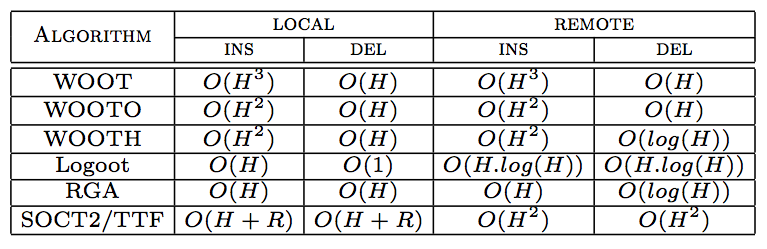
\includegraphics[width=0.7\textwidth]{includes/worst.png}
  \caption{Worst-case time-complexity analysis}
  \label{fig:worst}
\end{figure}